\cxset{%
 chapter opening=any,
 name=Chapter,
 numbering=arabic,
 number font-size=HHUGE,
 number font-family=rmfamily,
 number font-weight=bfseries,
 number before=,
 number dot=,
 number after=,
 number position= rightname,
 number display=block,
 number float=right,
 chapter display=block,
 chapter float=right,
 chapter font-family=\sffamily,
 chapter font-size=\Large,
 chapter before={\offinterlineskip\hbox{\vrule height2pt width\textwidth}\vskip3.5pt}\hfill,
 chapter after=\vskip3.5pt,
 chapter color=black!90,
 number color=black!90,
 chapter title width={0.5\textwidth},
 title margin-left=0pt,
 chapter title align=right,
 chapter title text-align=raggedleft,
 chapter margin top=0pt,
 chapter margin-left=0pt,
 title margin top=0pt,
 title margin bottom=10pt,
 title before={},
 title after={},
 title font-family=sffamily,
 title font-color=black!90,
 title font-weight=bfseries,
 title font-size=LARGE,
 section numbering prefix=\thechapter.,
 section color=black,
 subsection color=black}
 
\chapter{Review of Basic Fluid Mechanics Concepts}
\thispagestyle{headings}

This book is $5.51\times9.06$ inches and was produced according with the soft copy I have with Acrobat Distiller 5.0 (Windows). It uses a variety of fonts Arial, Century Schoolbook and Helvetica, Times Roman, MathematicalPi-One.
\medskip
\begin{figure}[ht]
\centering
\fbox{%
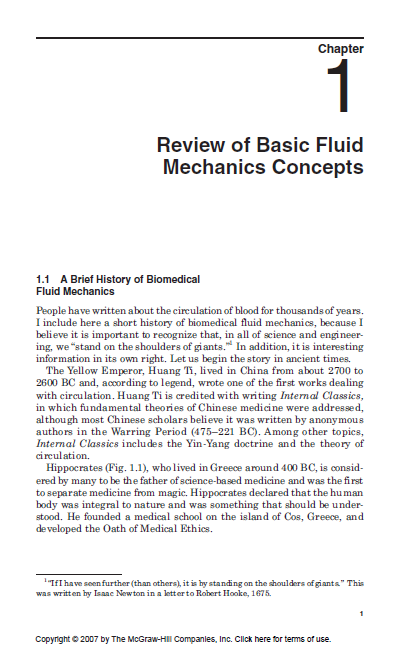
\includegraphics[width=0.45\textwidth]{./chapters/chapter14}
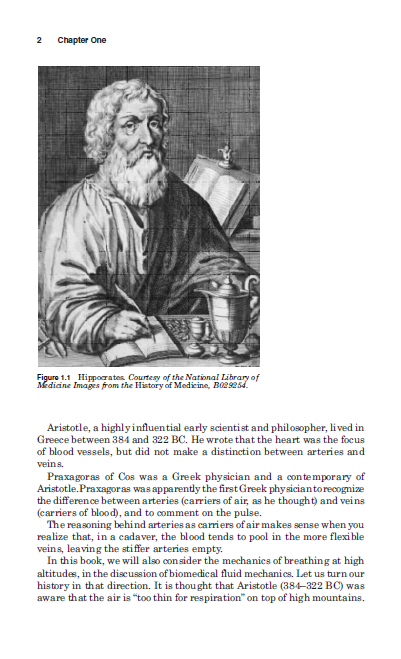
\includegraphics[width=0.45\textwidth]{./chapters/chapter14a.png}}
\end{figure}
\lipsum[2]

\section{Images}

\begin{figure}[ht]
\centering
\includegraphics[width=0.8\textwidth]{biofluids}
\end{figure}
\lipsum[2]

\lipsum[1]
\section{Examples}
Both full page ad well as block examples exist, these are all in boxes and they are numbered either with subsection counters in a fashion that is continuous from the text. 
\begin{figure}[ht]
\centering
\includegraphics[width=0.8\textwidth]{biofluids-1}
\end{figure}
\lipsum[2-4]

\begin{figure}[!b]
\begin{scriptexample}{This is a test}{}
\subsection{Clinical feature: polycythemia}

Polycythemia refers to a condition in which there is an increase in hemoglobin
above 17.5 g/dL in adult males or above 15.5 g/dL in females
(Hoffbrand and Pettit, 1984). There is usually an icrease in the number of
red blood cells above 6 - 1012 $L{^1}$ in males and 5.5 - 1012 $L^{-1}$ in females.
That is, a sufferer from this condition has a much higher blood viscosity due
to this elevated red blood cell count.
\end{scriptexample}
\end{figure}

Our boxes with the \pkgname{tcolorbox} are more than adequate for the job. The color settings can be changed via normal tcolorbox key settings that I have linked to the phd package keys.

The boxes can be also turned into floating boxes and to force them either to be on a full page or at the bottom in order for them to make a better impact in the layout. Key settings for setting the color of the boxes are provided
as well as a special environment.

\begin{verbatim}
\cxset{example box color=thegray}
\end{verbatim}

These example or sideboxes can easily be modified and you may have to provide your own, if you want anything particularly fancy. See the tcolorbox manual for many setting, but please do not use rounded boxes. 
%\end{document}